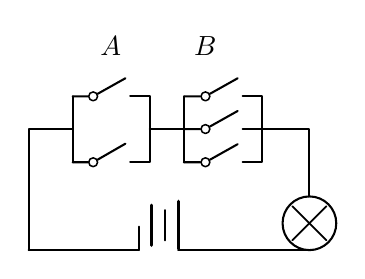
\begin{tikzpicture}[x=.62cm,y=.62cm,line cap=round,line join=round,baseline=(current bounding box.center)]
  \tikzset{contact/.style={circle,draw,line width=.55pt,fill=white,inner sep=0pt,minimum size=3.2pt}}
  \draw[line width=.75pt] (0,0)--(0,2.48)--(.90,2.48);
  \draw[line width=.75pt] (.90,1.80)--(.90,3.15);
  \node[contact] (a1) at (1.32,3.15) {}; \node[contact] (a2) at (1.32,1.80) {};
  \draw[line width=.75pt] (.90,3.15)--(a1)--(1.98,3.52);
  \draw[line width=.75pt] (.90,1.80)--(a2)--(1.98,2.18);
  \draw[line width=.75pt] (2.08,3.15)--(2.48,3.15)--(2.48,1.80)--(2.08,1.80);
  \draw[line width=.75pt] (2.48,2.48)--(3.18,2.48);
  \draw[line width=.75pt] (3.18,1.80)--(3.18,3.15);
  \node[contact] (b1) at (3.62,3.15) {}; \node[contact] (b2) at (3.62,2.48) {}; \node[contact] (b3) at (3.62,1.80) {};
  \draw[line width=.75pt] (3.18,3.15)--(b1)--(4.28,3.52);
  \draw[line width=.75pt] (3.18,2.48)--(b2)--(4.28,2.85);
  \draw[line width=.75pt] (3.18,1.80)--(b3)--(4.28,2.17);
  \draw[line width=.75pt] (4.38,3.15)--(4.78,3.15)--(4.78,1.80)--(4.38,1.80);
  \draw[line width=.75pt] (4.38,2.48)--(4.78,2.48)--(5.75,2.48)--(5.75,1.10);
  \draw[line width=.75pt] (5.75,0)--(3.06,0);
  \draw[line width=.75pt] (0,0)--(2.25,0);
  \draw[line width=.75pt] (2.25,0)--(2.25,.48); \draw[line width=1.15pt] (2.52,.10)--(2.52,.92); \draw[line width=.75pt] (2.79,.20)--(2.79,.82); \draw[line width=1.15pt] (3.06,.03)--(3.06,1.00);
  \draw[line width=.75pt] (5.75,.55) circle (.55); \draw[line width=.65pt] (5.40,.20)--(6.10,.90); \draw[line width=.65pt] (5.40,.90)--(6.10,.20);
  \node[above] at (1.68,3.78) {$A$}; \node[above] at (3.62,3.78) {$B$};
\end{tikzpicture}
